\documentclass[12pt,a4paper]{article}
\usepackage[utf8]{inputenc}
\usepackage[T1]{fontenc}
\usepackage{amsmath}
\usepackage{amsfonts}
\usepackage[francais]{babel}
\usepackage{amssymb}
\usepackage{graphicx}
\usepackage[top=2.00cm]{geometry}
\usepackage{enumitem}
\usepackage{tikz}
\usepackage{mathtools}
\usepackage{pgfplots}
\usepackage{textcomp}
\usepackage{pdflscape}
\usetikzlibrary{plotmarks}
\usepackage{bigcenter}
\usepackage{multicol}
\date{19 novembre 2016}
%Modif des enumerates numeros en gras. leftmargin=*,
\setlist[enumerate]{label=\textbf{\arabic*}.}

\usepackage{titlesec}
%modif des titres de section diminuer la taille
\titleformat{\section}
  {\normalfont\fontsize{14}{15}\bfseries}{\thesection}{1em}{}
\titleformat{\subsection}
  {\normalfont\fontsize{12}{15}\bfseries}{\thesubsection}{1em}{}

\pgfplotscreateplotcyclelist{styleWithoutError}{%
blue,every mark/.append style={fill=blue!80!black},mark=*\\%
red,every mark/.append style={fill=red!80!black},mark=square*\\%
brown!60!black,every mark/.append style={fill=brown!80!black},mark=otimes*\\%
black,mark=star\\%
blue,every mark/.append style={fill=blue!80!black},mark=diamond*\\%
red,densely dashed,every mark/.append style={solid,fill=red!80!black},mark=*\\%
brown!60!black,densely dashed,every mark/.append style={
solid,fill=brown!80!black},mark=square*\\%
black,densely dashed,every mark/.append style={solid,fill=gray},mark=otimes*\\%
blue,densely dashed,mark=star,every mark/.append style=solid\\%
red,densely dashed,every mark/.append style={solid,fill=red!80!black},mark=diamond*\\%
}
\pgfplotscreateplotcyclelist{styleWithError}{%
blue,every mark/.append style={fill=blue!80!black},mark=*,error bars/.cd,y dir=both, y explicit,x dir=both, x explicit,error mark=none\\%
red,every mark/.append style={fill=red!80!black},mark=square*,error bars/.cd,y dir=both, y explicit,x dir=both, x explicit,error mark=none\\%
brown!60!black,every mark/.append style={fill=brown!80!black},mark=otimes*,error bars/.cd,y dir=both, y explicit,x dir=both, x explicit,error mark=none\\%
black,mark=star,error bars/.cd,y dir=both, y explicit,x dir=both, x explicit,error mark=none\\%
blue,every mark/.append style={fill=blue!80!black},mark=diamond*,error bars/.cd,y dir=both, y explicit,x dir=both, x explicit,error mark=none\\%
red,densely dashed,every mark/.append style={solid,fill=red!80!black},mark=*,error bars/.cd,y dir=both, y explicit,x dir=both, x explicit,error mark=none\\%
brown!60!black,densely dashed,every mark/.append style={
solid,fill=brown!80!black},mark=square*,error bars/.cd,y dir=both, y explicit,x dir=both, x explicit,error mark=none\\%
black,densely dashed,every mark/.append style={solid,fill=gray},mark=otimes*,error bars/.cd,y dir=both, y explicit,x dir=both, x explicit,error mark=none\\%
blue,densely dashed,mark=star,every mark/.append style=solid,error bars/.cd,y dir=both, y explicit,x dir=both, x explicit,error mark=none\\%
red,densely dashed,every mark/.append style={solid,fill=red!80!black},mark=diamond*,error bars/.cd,y dir=both, y explicit,x dir=both, x explicit,error mark=none\\%
}


\author{CHARNAY Valentin, FINOT Sylvain}
\title{Compte rendu de TP : \\ Étude du point critique de l'Hexafluorure de Soufre }

\begin{document}
\maketitle
L'objectif de ce TP est d'effectuer une étude du point critique à l'aide d'un appareil qui permet d'obtenir les courbes isothermes dans le diagramme de phases (courbes d'Andrews). 
\section{RÉSEAU D'ISOTHERMES – APPLICATIONS}
\subsection{Mesure à effectuer}
Dans cette partie du T.P, on construit le réseau d'isothermes de SF$_{6}$.
Nous avons réalisé une série de mesures, toutes espacées d'environ 5K. Nous avons utilisé Regressi pour exploiter les données et tracer les différents diagrammes (Amagat, Clapeyron etc). Les incertitudes calculées seront basées sur les incertitudes suivantes :
\begin{center}
\begin{tabular}{|c|c|c|}
\hline
$\Delta$T & $\Delta$P & $\Delta$V \\ \hline
0,1K      & 0,5bar       & $5.10^{-2}$mL       \\ \hline
\end{tabular}
\end{center}

\subsection{Utilisation du diagramme de Clapeyron}

\begin{enumerate}
\item On remarque que pour la majorité des courbes ($T<T_{c}$), on peut distinguer très nettement trois phases (classées par ordre décroissant de volume) :

\begin{itemize}[label=\textbullet]
\item la pression croit lentement, présence d'une seule phase (gazeuse).
\item plateau horizontal, caractérisé par le fait que la pression reste constante à partir de l'apparition de la première goutte de liquide et ce jusqu'à la disparition de la dernière bulle de gaz.
\item Brusque augmentation de la pression, en effet un liquide est très peu / incompressible.
\end{itemize}

La température critique correspond à la température pour laquelle il n'y a plus de plateau à pression constante. On en déduit alors la Pression et le Volume critique.
Dans nôtre cas, le point serait entre T=318K, V=0,4 mL, P=38 bar et T=323 K, V=0,4 mL, P=41 bar.
Il aurait fallu refaire une série de mesure à température intermédiaire pour le déterminer avec précision.\\
Après une petite recherche, le point critique de SF$_{6}$ est T=318,7K et P=37,6 bar. Notre mesure a 318K était relativement proche du point critique, quant à celle a T=323K, nous l'avions déjà dépassé.
 
\item On a tracé la courbe de pression de vapeur saturante sur le diagramme de Clapeyron, celle ci est nommée "Courbe de PVS" dans la légende. \\
La phase liquide se trouve à sa gauche, la partie biphasée est entre l'axe des abscisse et la courbe et la phase gazeuse est à sa droite.

\item Chaleur latente. \\
La expression de la chaleur latente est donnée par la formule de Clausius-Clapeyron : \[L=T.\dfrac {dP_{Sat}} {dT}.(v_{gaz}-v_{liq})\]
Remarque : La chaleur latente devrait s’annuler au point critique puisque qu'en ce point, $(v_{gaz}-v_{liq})=0$ (les propriété du liquide sont très proches de celle du gaz en ce point.)  \\
Il nous faut donc déterminer $\dfrac {dP_{Sat}} {dT}$, pour cela nous avons fait une régression linéaire de la fonction $P_{Sat}=f(T)$\\
\begin{center}
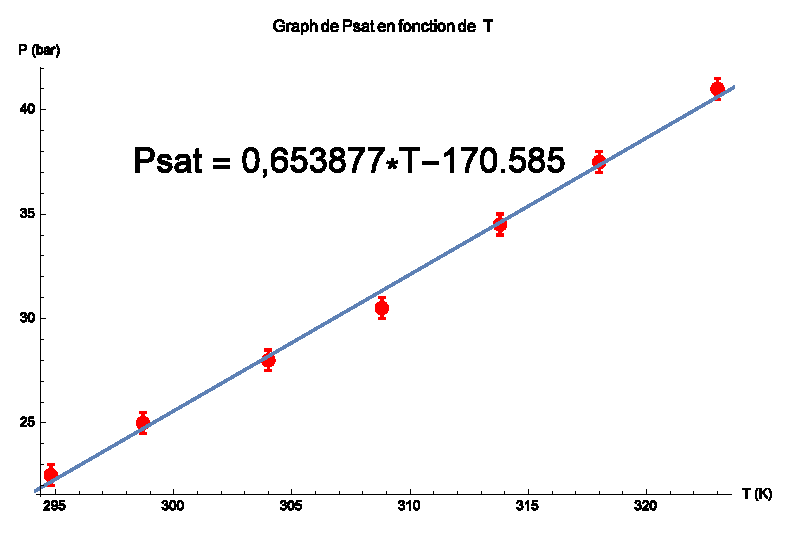
\includegraphics[scale=0.75]{RegressionPsat.eps}
%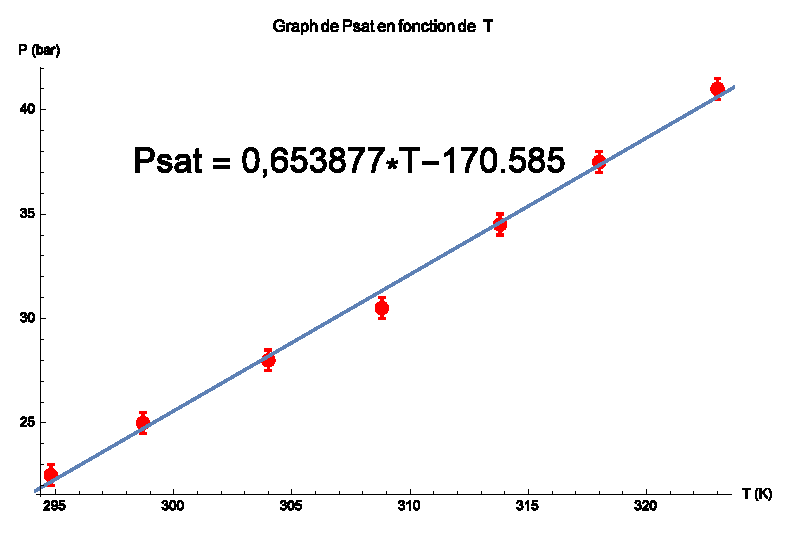
\includegraphics[scale=0.4]{RegressionPsat}
\end{center}
On remarque que la régression est plutôt bonne.
Nous avons donc la valeur de $\dfrac {dP_{Sat}} {dT}=0,6539.10^{5} $Pa/K\\
Calculons Q(T)=n.L(T) (i.e on remplace les volumes molaires).
On essaye aussi d'approximer le nombre de mole de gaz en utilisant le modèle des gaz parfaits.

\begin{align}
Q(T)&=T.\dfrac {dP_{Sat}} {dT}.(V_{gaz}-V_{liq})\\
n&=\dfrac{P.V_{g}}{R.T} \\
L&=\dfrac{Q}{n.M_{SF_{6}}} \quad \text{avec} \quad M_{SF_{6}}=146.06 g.mol^{-1}
\end{align}

\begin{center}
\begin{tabular}{|c|c|c|c|c|c|c|}
P & T & Vg & Vl & n & Q & L  \\ \hline
bar & K & mL & mL & mol & J & kJ.kg$^{-1}$  \\ \hline
22,50 & 294,8 & 1,250 &  0,3000 & 0,001148 & 18,31 & 109,3 $\pm  14$  \\ \hline
25,00 & 298,7 & 1,100 &  0,3000 & 0,001107 & 15,90 & 96,61 $\pm 14$  \\ \hline
28,00 & 304,0 & 0,9500 &  0,3000 & 0,001052 & 12,92 & 84,09 $\pm 15$  \\ \hline
30,50 & 313,8 & 0,8000 &  0,3000 & 0,0009352 & 10,26 & 75,14 $\pm 17$  \\ \hline
37,50 & 318,0 & 0,6500 &  0,3000 & 0,000922 & 7,278 & 54,07 $\pm 18$\\  \hline
\end{tabular}
\end{center}
On trouve environ $1,1.10^{-3}$ mol et une chaleur latente (à 298,7K et 25bar) de 96,61 $\pm14$ kJ.kg$^{-1}$. Cette dernière valeur est éloignée des 166kJ.kg$^{-1}$ donnée à 298k sous une pression de 1bar. Cette différence est peut être du au fait que l'approximation des gaz parfaits soit mauvaise, ou au fait que la valeur est donnée à 1bar alors que nous l'avons calculée à 25bar.
\end{enumerate}

\subsection{Utilisation du diagramme d'Amagat}
Dans le diagramme d’Amagat PV = f(P) les isothermes d'un gaz parfait sont des droites horizontales (PV=nRT avec nRT=cst).
Dans notre cas (voir graphique) :
\begin{itemize}
\item lorsque P est faible, le diagramme d’Amagat possède une allure de droite affine avec une pente faible  $\approx$ Gaz Parfait.
\item Le plateau horizontal lors du changement de phase présent dans le diagramme de Clapeyron devient une droite verticale de pente infinie. En effet P reste constant mais V diminue lors de la condensation. Le produit PV diminue à P=cst.
\item Nous n'avons pas pris suffisamment de point à haute pression pour observer correctement la troisième partie du diagramme d'Amagat. Nous devrions logiquement observer une augmentation rapide du  lorsque SF$_{6}$ est entièrement sous forme liquide (i.e incompressible). Le volume ne diminue (presque) plus lorsque P augmente.
\end{itemize}    


Par régression linéaire des mesures effectuées à pressions "relativement" faibles (P<16bar), on essaye d'approximer n. La régression nous donne une équation affine : $PV=a*P+b$, ainsi en approximant a un gaz parfait on obtient : \[\lim_{P \to 0} PV = b \stackrel{\text{GP}}{=} nRT \quad \implies n=\dfrac{b}{R.T}\]
\begin{center}
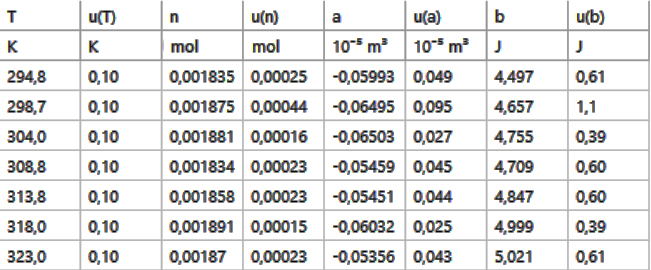
\includegraphics[scale=0.5]{nAmagat}\\
\end{center}
On peut alors encadrer la valeur de n.\\ n=$1,8.10^{-3}\pm{4.10^{-4}}$mol\\
Cette valeur est relativement éloigné des  1,1.10$^{-3}$ trouvé en approximant avec le modèle des gaz parfaits. Il se pourrait donc que l'approximation soit mauvaise.

\subsection{Coefficients du viriel}
L'équation d'état d'un gaz réel peut s'exprimer sous la forme de
développement en série d'une variable : \[PV=nRT\left( 1+\dfrac {B_{0}} {V}+\dfrac {B_{1}} {V^{2}}+\dfrac {B_{2}} {V^{3}}+...\right)\]
Nous pouvons remarquer qu'au premier ordre \[\lim_{1/V \to 0} PV = nRT\left( 1+\dfrac {B_{0}} {V}\right)\]Autrement dit, il s'agit d'une droite d'équation : 
\[
\begin{aligned}
f(\dfrac{1}{V})=A*\dfrac{1}{V}+C \quad \text{avec} \quad A=nRT.B_{0} \quad C=nRT
\end{aligned}
\]

Sur le diagramme PV en fonction de 1/V, on constate que les courbes au-dessus de la courbe de saturation ont un comportement affine. Ce qui correspond bien avec notre approximation. Quant à la partie des courbes en dessous de la courbe de saturation, elles ressemblent d'avantage à des paraboles $\implies$ le terme $\dfrac{B_{1}}{V^{2}}$ n'est plus négligeable devant le terme $\dfrac{B_{0}}{V}$ \\
Remarque : On peut recalculer le nombre de mole de gaz $n=\dfrac{C}{RT}$\\
Calculons le premier coefficient de viriel pour chaque température : 
$B_{0}=\dfrac{A}{C}$\\
Par la suite on trace B$_{0}$(T), on remarque alors que ce dernier est de la forme : a*T+c. On peut alors supposer que les autres coefficients B$_{i}$ ne dépendent eux aussi que de la température. 
%\section{LE POINT CRITIQUE}
%\subsection{Opalescence critique}
%Comme cité dans notre sujet : 
%\begin{quotation}
%La présence d'irrégularités de densité au sein d'un milieu provoque la diffusion de la lumière.
%Or au voisinage des conditions critiques, de fortes fluctuations de densité se manifestent dans les fluides. L'intensité de la lumière diffusée est une fonction fortement décroissante de la
%longueur d'onde (de l'ordre de $1/\lambda^{4}$)
%\end{quotation}
%Ce qui ce traduit par la diffusion des plus courtes longueurs d'ondes correspondant au bleu dans le visible. C'est le phénomène de l'opalescence critique.

\pagebreak
\begin{bigcenter}
\begin{multicols}{2}
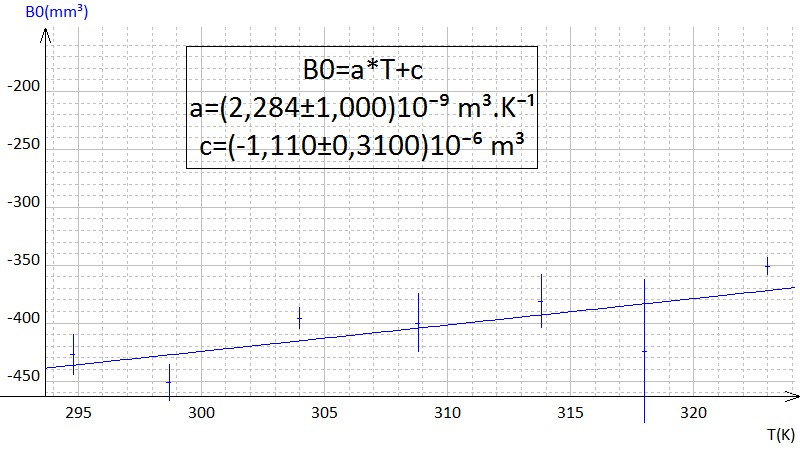
\includegraphics[height=6cm]{B0(T)}
\columnbreak
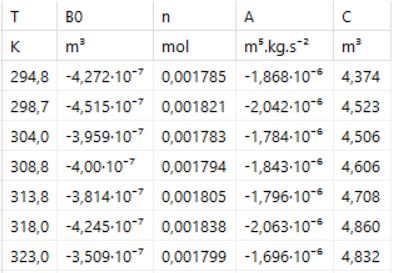
\includegraphics[height=6cm]{Viriel}
\end{multicols}
\end{bigcenter}

\begin{center}

\begin{tikzpicture}
\begin{axis}[
height=8cm,width=12cm
,axis x line=bottom,axis y line=left
,xmin=0.06,xmax=5.19
,ymin=0.082638592,ymax=4.462206208
,title={PV=f(1/V) }
,xlabel={1/V(cm$^{-3}$)}
,ylabel={PV(J)}
]
\addplot[draw=red
] file
 {viriel10.txt};
\addplot[draw=red
] file
 {viriel11.txt};
\addplot[draw=red
] file
 {viriel12.txt};
\addplot[draw=red
] file
 {viriel13.txt};
\addplot[draw=red
] file
 {viriel14.txt};
\addplot[draw=red
] file
 {viriel15.txt};
\addplot[draw=red
] file
 {viriel16.txt};
\addplot[draw=black, dashed
,mark=x
] file
 {viriel17.txt};
\end{axis}
\end{tikzpicture}
\begin{tikzpicture}
\begin{axis}[
height=8cm,width=12cm
,axis x line=bottom,axis y line=left
,xmin=0,xmax=5.2
,ymin=0,ymax=4.472
,grid=major
,title={Modele affine pour 1/V $\rightarrow$ 0 }
,xlabel={1/V(cm$^{-3}$)}
,ylabel={PV(J)}
]
\addplot[draw=red
,only marks
,mark=x
] file
 {viriel20.txt};
\addplot[draw=red
,mark=none,smooth
] file
 {viriel22.txt};
\addplot[draw=red
,mark=none,smooth
] file
 {viriel23.txt};
\addplot[draw=red
,only marks
,mark=x
] file
 {viriel24.txt};
\addplot[draw=red
,mark=none,smooth
] file
 {viriel26.txt};
\addplot[draw=red
,mark=none,smooth
] file
 {viriel27.txt};
\addplot[draw=red
,only marks
,mark=x
] file
 {viriel28.txt};
\addplot[draw=red
,mark=none,smooth
] file
 {viriel210.txt};
\addplot[draw=red
,mark=none,smooth
] file
 {viriel211.txt};
\addplot[draw=red
,only marks
,mark=x
] file
 {viriel212.txt};
\addplot[draw=red
,mark=none,smooth
] file
 {viriel214.txt};
\addplot[draw=red
,mark=none,smooth
] file
 {viriel215.txt};
\addplot[draw=red
,only marks
,mark=x
] file
 {viriel216.txt};
\addplot[draw=red
,mark=none,smooth
] file
 {viriel218.txt};
\addplot[draw=red
,mark=none,smooth
] file
 {viriel219.txt};
\addplot[draw=red
,only marks
,mark=x
] file
 {viriel220.txt};
\addplot[draw=red
,mark=none,smooth
] file
 {viriel222.txt};
\addplot[draw=red
,mark=none,smooth
] file
 {viriel223.txt};
\addplot[draw=red
,only marks
,mark=x
] file
 {viriel224.txt};
\addplot[draw=red
,mark=none,smooth
] file
 {viriel226.txt};
\addplot[draw=red
,only marks
,mark=x
] file
 {viriel227.txt};
\end{axis}
\end{tikzpicture}
\end{center}

\begin{landscape} % % Diagramme de Clapeyron
\thispagestyle{empty}
%\parindent=0pt
%\eject\null
%\vfill
\hspace*{-4cm}
\vspace*{-2cm}
\centering
%\begin{bigcenter}
\begin{tikzpicture}
\begin{axis}[
height=16cm,width=20cm
,axis x line=bottom,axis y line=left
,xmin=0.048,xmax=2.06340740740741
,ymin=15.8368749635271,ymax=46.097571883008
,grid=major
,title={Diagramme de Clapeyron P(V) }
,xlabel={V(cm$^{3}$)}
,ylabel={P(bar)}
,legend entries={Courbe de PVS,T=294.8K,T=298.7K,T=304K,T=308.8K,T=313.8K,T=318K,T=323K}
,cycle list name=styleWithError
]
\addplot[draw=gray, smooth] file
 {Sat.txt};
\addplot table[x error index=2,y error index=3]
 {Clapeyron10.txt};
\addplot table[x error index=2,y error index=3]
 {Clapeyron11.txt};
\addplot table[x error index=2,y error index=3]
 {Clapeyron12.txt};
\addplot table[x error index=2,y error index=3]
 {Clapeyron13.txt};
\addplot table[x error index=2,y error index=3]
 {Clapeyron14.txt};
\addplot table[x error index=2,y error index=3]
 {Clapeyron15.txt};
\addplot table[x error index=2,y error index=3]
 {Clapeyron16.txt};
\end{axis}
\end{tikzpicture}
\end{landscape}

\begin{landscape} % %Diagramme d'Amagat
\thispagestyle{empty}
%\parindent=0pt
%\eject\null
%\vfill
\hspace*{-4cm}
\vspace*{-2cm}
\centering
\begin{tikzpicture}
\begin{axis}[
height=16cm,width=20cm
,axis x line=bottom,axis y line=left
,xmin=9.11720348442624,xmax=45.5255295587628
,ymin=0.313110115854757,ymax=4.8792993054033
,grid=major
,title={Diagramme d'Amagat }
,xlabel={P(bar)}
,ylabel={PV(J)}
,legend entries={,T=294.8K,T=298.7K,T=304K,T=308.8K,T=313.8K,T=318K,T=323K}
,cycle list name=styleWithError
]
\addplot table[x error index=2,y error index=3]
 {Amagat10.txt};
\addplot table[x error index=2,y error index=3]
 {Amagat11.txt};
\addplot table[x error index=2,y error index=3]
 {Amagat12.txt};
\addplot table[x error index=2,y error index=3]
 {Amagat13.txt};
\addplot table[x error index=2,y error index=3]
 {Amagat14.txt};
\addplot table[x error index=2,y error index=3]
 {Amagat15.txt};
\addplot table[x error index=2,y error index=3]
 {Amagat16.txt};
\end{axis}
\end{tikzpicture}
\end{landscape}



\end{document}
